\chapter{Pražská Integrovaná doprava (PID)}
\label{3-teorie-pid}

Pražská integrovaná doprava (\zk{PID}) je dopravní systém, který zahrnuje jak pozemní
dopravu (tramvaje, železnici, městské a příměstské autobusové linky, lanovou dráhu na Petřín),
tak i tu podzemní (metro). Tento dopravní systém zahrnuje i některé přívozy. 
Systém probíhá integrací společnými přepravními a tarifními podmínkami a jednotným dopravním řešením včetně 
koordinace jízdních řádů. \cite{pid}
\vskip 0.2in
 
\begin{figure}[H] \centering
    
\includegraphics[width=400pt]{./pictures/pid-logo.png}
    \caption[Logo Pražské integrované dopravy]{Logo Pražské integrované dopravy \cite{pid}}
	\label{fig:pid-logo}                                
\end{figure} 

\section{ROPID}

Chod integrace systému zajišťuje Regionální organizátor pražské integrované dopravy (zkráceně ROPID),
což je příspěvková organizace hlavního města Prahy. Jeho úloha je organizační a kontrolní
a ze své práce se odpovídá orgánům samosprávy a státní správy, které jej zabezpečením dopravy pověřily.

\begin{figure}[H] \centering
    
\includegraphics[width=200pt]{./pictures/ropid-logo.jpg}
    \caption[Logo organizace ROPID]{Logo organizace ROPID \cite{pid}}
	\label{fig:ropid-logo}                                
\end{figure}

ROPID se zabývá vytvářením, rozvíjením a udržováním systému Pražské integrované dopravy v Praze a okolí,
včetně návazností na jiné systémy jako jsou Integrovaná doprava Plzeňského kraje,
Doprava Ústeckého kraje, Integrovaný dopravní systém Libereckého kraje nebo 
Integrovaná regionální doprava Královéhradeckého a Pardubického kraje.
Taktéž se zabývá vytvářením zásad a standardů dopravní obsluhy a jejich aplikace v závislosti
na dostupných finančních zdrojích a jejich projednání s obcemi, okresními úřady a dopravci.
ROPID vybírá dopravce, uzavírání smluv o závazku veřejné služby jménem města Prahy 
k zajištění provozu \zk{PID} s dotčenými obcemi, Středočeským krajem a dopravci a kontrola jejich plnění.
Náplní organizace ROPID jsou i uspořádání finančních toků v systému \zk{PID}, návrh tarifů a jízdného v systému \zk{PID} a
zajištění jednotnosti informačního systému \zk{PID}.  \cite{wikipedia-ropid}

\section{Tarifní pásma PID}
                    
Tzv. \uv{tarifní pásma} je rozdělení Pražské integrované dopravy do zón, kde v jednotlivých
zónách platí rozdílné cenové podmínky. Rozdělení tarifních pásem je následující:
P, 0, B, 1, 2, 3, 4, 5, 6, 7, 8, 9. Tarifní pásma P, 0 a B se nacházejí v Praze a územně
se spolu překrývají. Ostatní pásma (1 až 9) se z větší části nacházejí ve Středočeském kraji a z
menší části v Plzeňském kraji, Ústeckém kraji a na Vysočině.

Do pásma P jsou zařazeny všechny linky metra, tramvají, městských autobusů, přívozů,
včetně lanové dráhy na Petřín a vybraných železničních stanic a zastávek v centru Prahy.
Pásmo P má dvojnásobnou tarifní hodnotu (tj. je počítáno jako dvě tarifní pásma).
Do pásma 0 jsou zařazeny dojezdové úseky příměstských autobusových linek a vybrané
železniční stanice a zastávky v širší oblasti okolo centra Prahy.
Do pásma B jsou zařazeny úseky příměstských autobusových linek a vybrané 
železniční stanice a zastávky v okrajových částech Prahy. \cite{pid} 

Pro pásma nacházející se ve Středočeském kraji jsou zařazeny jednotlivé stanice 
a zastávky příměstských autobusových linek \zk{PID} a vlaků zahrnutých do \zk{PID}. 
Příslušnost stanice nebo zastávky k tarifnímu pásmu je vždy dána jízdním řádem konkrétní linky.\cite{pid}

\begin{figure}[H] \centering
    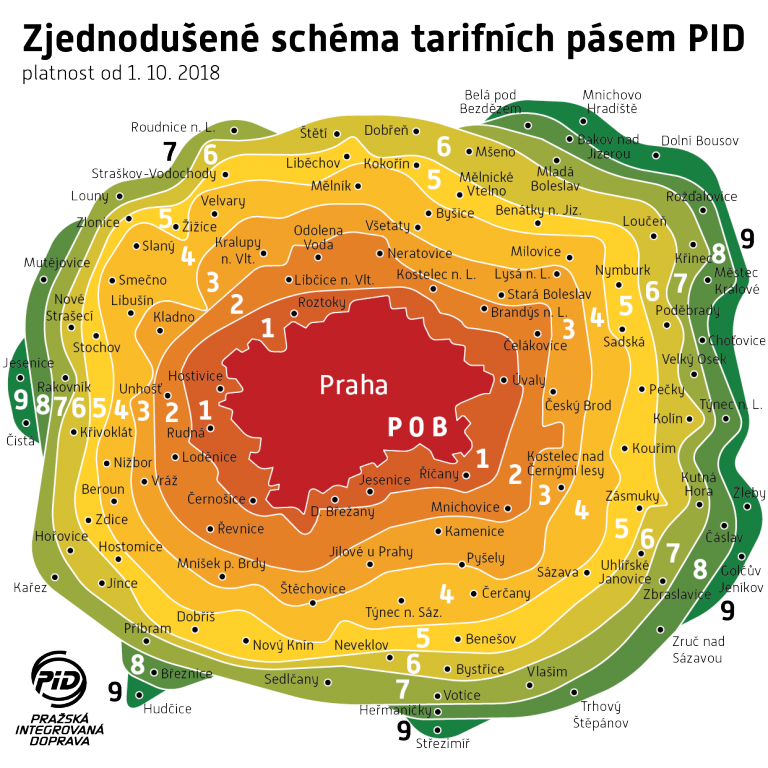
\includegraphics[width=400pt]{./pictures/pasma-schema.png}
    \caption[Schéma tarifních pásem \zk{PID}]{Schéma tarifních pásem \zk{PID} \cite{pid}}
	\label{fig:pasma-schema}                                
\end{figure}

\subsection{Tvorba tarifních pásem PID}

Tarifní pásma Pražské integrované dopravy se tvoří téměř celá manuálně. Zeptal jsem
se tedy paní Ing. Zuzany Šaškové z ROPIDu, která se tvorbou pásem zabývá, jakou metodiku
při tom používá. 

%% ML: nasledujici odstavec autorizujte u pani Saskove...
Paní Ing. Šašková používá na úpravu dat software ArcMap od společnosti Esri.
\textit{\uv{Původní myšlenka při tvorbě tarifních pásem byla zohledňovat v mapě 
zastavěná území obce tak, aby je tarifní pásma pokud možno neprotínala,}} od této
myšlenky ustoupila kvůli náročnosti zpracování. \textit{\uv{Dnes mám vytvořeny polygony 
jednotlivých pásem (nikoliv donuty), každé pásmo ručně upravím dle aktuálních změn.}}
V projektu při úpravách pracuje s jednoduchými nástroji, používá symbologii k \uv{obarvení}
zastávek a jednotlivých polygonů tarifního pásma stejnou barvou, hraniční zastávek výraznou barvou 
případně pro následné úpravy. \textit{\uv{Když ručně vytvaruji všechny polygony tak, aby procházely 
mezi zastávkami, které mají přiřazené jedno pásmo a skrz zastávky, které mají přiřazená dvě pásma,
pustím si skript Pythonu, který z polygonů vyřeže donuty jednotlivých tarifních pásem a nakonec je spojí do jedné vrstvy.}}

Takto paní Ing. Šašková upravuje tarifní pásma od dubna 2018 při každé úpravě zastávek. 
Zatímco dříve byla důležitá schématická verze mapy, v současnosti se připravuje on-line mapa \zk{PID}, u které již je zapotřebí, 
aby tarifní pásma odpovídala realitě a upravovala se v návaznosti na postup
integrace dalších oblastí Středočeského kraje do \zk{PID}.

Zde na obrázku \ref{fig:pasma-schema} je uvedena nejstarší dochovaná podoba pásem z dubna roku 2018.
Pro zajímavost si lze všimnout, že v té době tarifní pásmo 7 bylo poslední a všechna pásma tvarově připomínala
spíše tu schématickou verzi.

\begin{figure}[H] \centering
    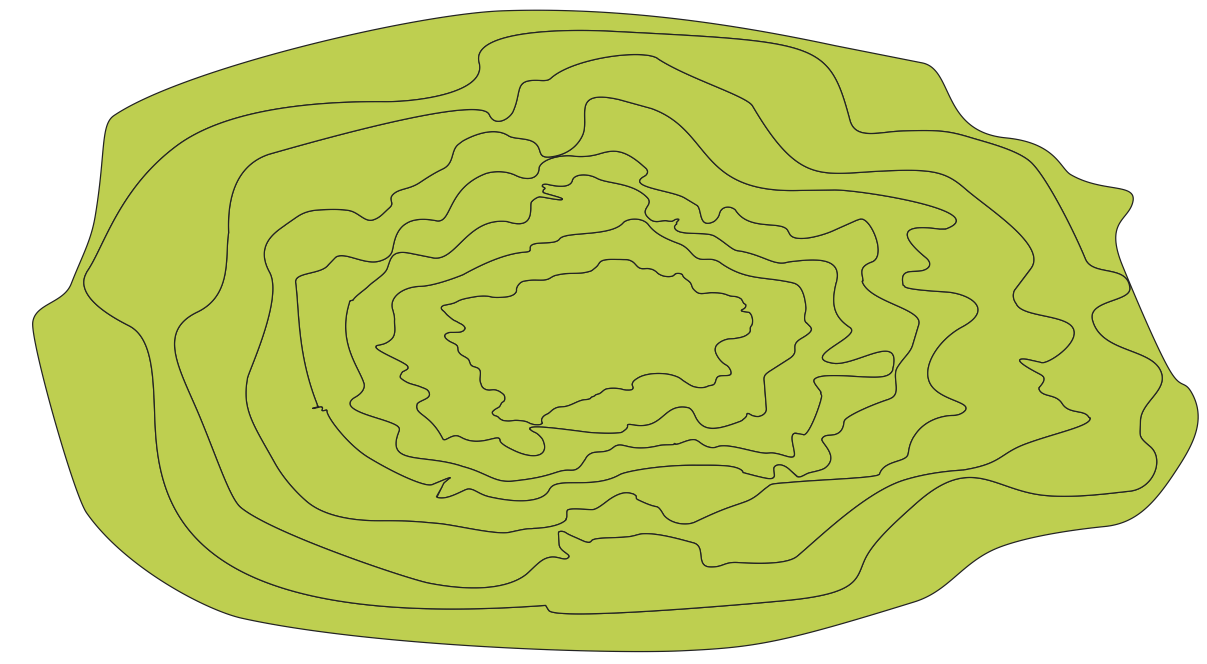
\includegraphics[width=400pt]{./pictures/pasma-nejstarsi.png}
    \caption[Nejstarší dostupná verze tarifních pásem \zk{PID}]{Nejstarší dostupná verze tarifních pásem \zk{PID}}
	\label{fig:pasma-nejstarsi}                                
\end{figure}

Jak již bylo zmíněno v kapitole \ref{0-reserse}, tak na portálu \textit{Opendata hlavního města Prahy}
je pravidelně zveřejňován tvar tarifních pásem. Nejnovější verzi zveřejnila organizace ROPID 8. září 2020.
Naopak první verze byla zveřejněna již 16. září 2016, bohužel tato verze nikde nebyla k nalezení.
Zde je alespoň zobrazena verze tarifních pásem z 8. září 2020, kde byly pro přehlednost 
přebrány barvy pásem z schématu od \zk{PID} (viz \ref{fig:pasma-schema})

\begin{figure}[H] \centering
    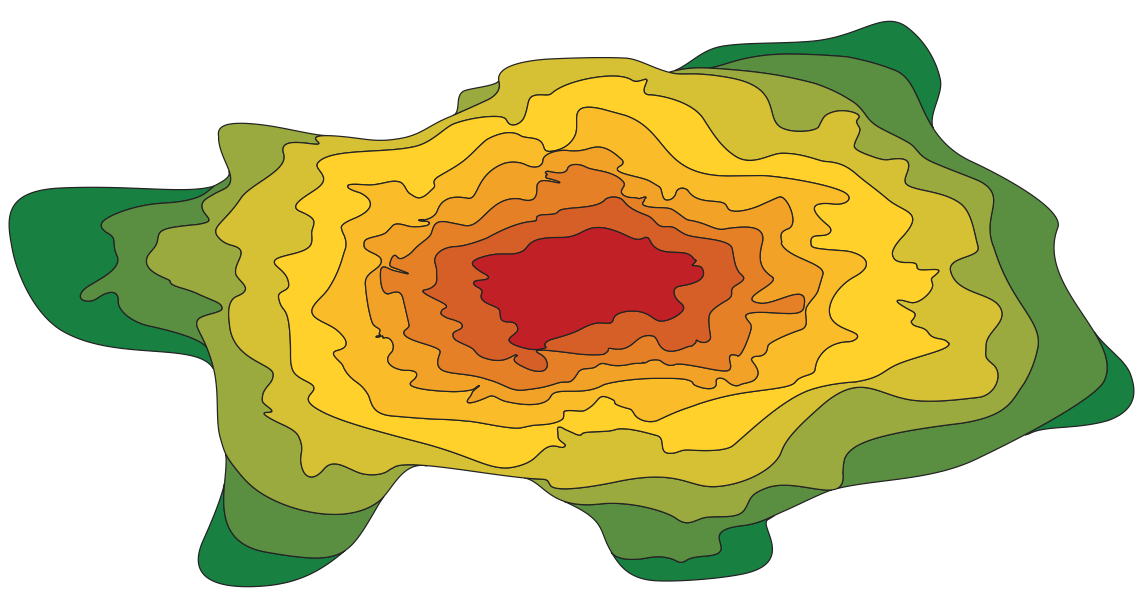
\includegraphics[width=400pt]{./pictures/pasma-ROPID.png}
    \caption[Tarifní pásma zveřejná organizací ROPID z 8. září 2020]{Tarifní pásma zveřejná organizací ROPID z 8. září 2020}
	\label{fig:pasma-ROPID}                                
\end{figure}


